\section{Application Planning and Requirements}
\subsection{Requirements and Specifications}
In the next subsection, this thesis will present a brief discussion regarding the possible stakeholder requirements alongside a more detailed specification list from the development perspective.

The act of stock market prediction is usually incorporated in large financial applications which may offer a variety of functionalities. However, in those applications the core functionalities are considered of a higher importance and relevance than the actual reliability of the prediction. This application will try to incorporate some functionalities from generic financial applications, while maintaining its core to the actual prediction and useful information along in order to facilitate decisions for the users (investors).

The application has to be easily accessible and offer the users a friendly and familiar environment. The user should be able to select a list of favorite companies to follow. For each company, he should be able to check details about the company, check the historical price and check prediction on both historical and future data. Moreover, the user should be linked with some recent financial news which might affect the market or to run a simulation on a given interval of time on historical data with a fixed investment strategy. Lastly, in order to encourage user engagement and provide a good experience, a feedback platform is mandatory for improving further the development. 

\vspace{5mm}

From the development perspective we have decided a list of specifications which should be fulfilled by the application. The application will have a sign-up and login system, using two types of users: client and admin with different permissions. Further, we'll split the specification list in two based on the role.

\paragraph{Client User}
\begin{itemize}
    \item List the available companies to follow
    \item List some recent news which might affect the future trend of the market
    \item Ability to select and add favorite companies
    \item Remove a company from your favorite list
    \item Request various details about a favorite company
    \item Request the historical data for a favorite company as a plot
    \item Request prediction for historical events to check the stability
    \item Request future prediction for the present moment for different time-horizons
    \item Run an investment simulation based on a set of companies and a fixed strategy
    \item Feedback report system to the developers
    \item Notification system regarding feedback answer
\end{itemize}

\paragraph{Admin User}
\begin{itemize}
    \item Create a new entity company with its details
    \item Update company details
    \item Update company networks links to make it available for the clients
    \item Remove a certain company from available companies for clients
    \item Respond to user feedback
    \item Request the system to update financial data available with new request from external API
\end{itemize}

\subsection{Application Architecture}
In order to facilitate accessibility for the application, the decided architecture is of type client-server where the client application will be a mobile application. This architecture was chosen with multiple reasons in mind while being known for its flexibility and allowing easily addition of different types of clients if necessary.

The need for a dedicated server (of sets of servers) stems firstly from the amount of financial data used for predictions. Bundling large amounts of data with a portable mobile application is unacceptable. Moreover, this data needs frequent updates from known sources which have free API-s available, but with some low limits of requests per day. In addition, a large amount of neural networks will be maintained for different goals, time-horizons and companies. While nowadays mobile phones are becoming more and more powerful being capable of running some machine learning tasks, still most of the work is done in the cloud on dedicated servers. Lastly, moving the computational cost from the client to a server allows the application to be run on a larger variety of devices which otherwise might have been insufficient.

In order to facilitate possible integration in modern cloud systems, we are going to split the server computation cost in two major parts. The first part which will directly communicate with the client application will contain the entire business logic necessary to address most features which do not require any sort of prediction. The second part will behave similar to a Cloud API service for machine-learning operations regarding stock market prediction. It will be standalone and totally separated from the first part, maintaining only the network architectures already trained and expose a REST API for the business logic server to request any computations regarding prediction. The following picture attached contains a visual description of what has been discussed.

\begin{figure}[H]
\centering
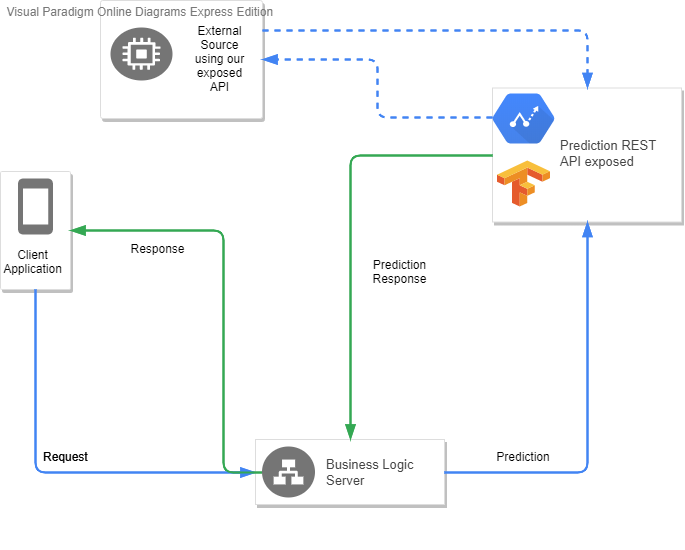
\includegraphics[height=12cm]{images/HighLevelArchitecture.png} 
\caption{High Level Architecture of the Application}
\label{fig:highlevelarchitecture}
\end{figure}


\subsection{Abstract Design - Use Case Diagram}
In the following subsection we are going to present the associated Use Case Diagram with the previously specified requirements specification. Two actors have been found along: the client and the admin. There are some use cases which belong to both, while most of them are separate.

\begin{figure}[H]
\centering
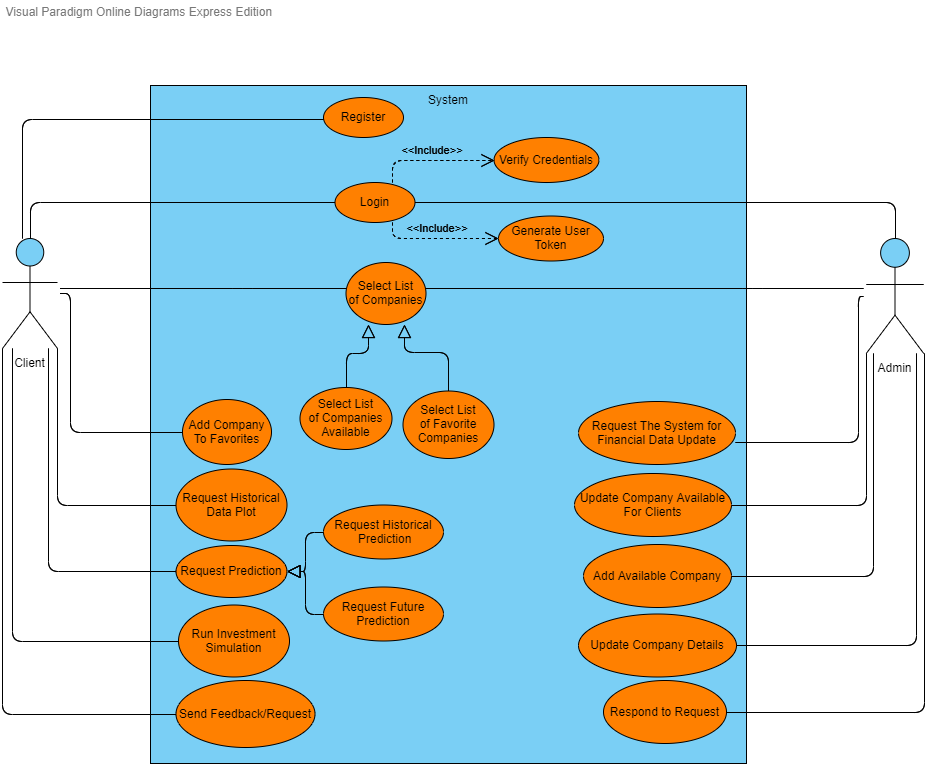
\includegraphics[height=13cm]{images/UseCaseDiagram.png} 
\caption{Use Case Diagram}
\label{fig:usecasediagram}
\end{figure}


\section{Application Core Functionalities}